\chapter{Discussion}
In this chapter, the results of experiments conducted in both simulation and on the real system are delved into. The chapter is structured as follows: The first section discusses the simulation leaderboard,the second section discusses the robustness leaderboard, and the third section discusses real hardware leaderboard. 

\section{Interpretation of simulation leaderboard}
In Table \ref{tab:performance_pendubot} and Table \ref{tab:performance_acrobot}, the performance leaderboard results for both the pendubot and acrobot in simulation experiments are presented. Three types of controllers are listed for comparison, namely model-free reinforcement learning(MFRL) based controller, model-based reinforcement learning(MBRL) based controller and trajectory based controller.

The SAC+LQR controller is our design and is a representative of model-free reinforcement learning method. 

MC-PILCO~\cite{amadio2022model}, which stands for Monte Carlo Probabilistic Inference for Learning Control, is a model-based reinforcement learning method. It utilizes probabilistic models to predict the system's dynamics and employs Monte Carlo methods to optimize control policies based on these predictions. This method was implemented by a team from the University of Padova~\cite{Libera2023AthleticIO}. 

tvLQR is an extension of the standard Linear Quadratic Regulator (LQR) control design. It is a trajectory based control method, tailored for systems with time-dependent state-space matrices or where the optimal control needs to be dynamic. Representing the optimal control method, it was implemented by a separate team from DFKI RIC\cite{2023_ram_wiebe_double_pendulum}.

% \begin{table}[H]
%   \centering
%  \begin{tabular}{lcccccc}
%  \hline
%  Criteria & \multicolumn{2}{c}{SAC+LQR} & \multicolumn{2}{c}{MC-PILCO} & \multicolumn{2}{c}{tvLQR} \\
%  & Pendubot & Acrobot & Pendubot & Acrobot & Pendubot & Acrobot \\
%  \hline
%  Swingup Success & success & success & success & success & success & success \\
%  Swingup time [s] & \textbf{0.65} & 2.06 & 1.43 & \textbf{1.1} & 4.2 & 3.98 \\
%  Energy [J] & 9.4 & 29.24 & 12.67 & \textbf{9.81} & \textbf{9.06} & 10.92 \\
%  Max. Torque [Nm] & 5.0 & 5.0 & \textbf{2.4} & \textbf{2.82} & 2.82 & 5.0 \\
%  Integrated Torque [Nm] & \textbf{2.21} & 4.57 & 3.48 & \textbf{1.27} & 2.57 & 2.27 \\
%  Torque Cost [N²m²] & 8.58 & 12.32 & 7.77 & \textbf{2.27} & \textbf{2.0} & 2.47 \\
%  Torque Smoothness [Nm] & 0.172 & 0.954 & 0.07 & \textbf{0.057} & \textbf{0.031} & 0.077 \\
%  Velocity Cost [m²/s²] & \textbf{44.98} & 193.78 & 94.68 & 242.44 & 137.31 & \textbf{100.34} \\
%  RealAI Score & 0.801 & 0.722 & \textbf{0.891} & \textbf{0.869} & 0.827 & 0.8 \\
%  \hline
%  \end{tabular}
%  \caption{Performance scores of various controllers for pendubot and acrobot experiments.}
%  \label{tab:performance_ideal}
% \end{table}

% Table for Pendubot results
\begin{table}[H]
  \centering
 \begin{tabular}{lccc}
 \hline
 Criteria & SAC+LQR & MC-PILCO & tvLQR \\
 \hline
 Swingup Success & success & success & success \\
 Swingup time [s] & \textbf{0.65} & 1.43 & 4.2 \\
 Energy [J] & 9.4 & 12.67 & \textbf{9.06} \\
 Max. Torque [Nm] & 5.0 & \textbf{2.4} & 2.82 \\
 Integrated Torque [Nm] & \textbf{2.21} & 3.48 & 2.57 \\
 Torque Cost [N²m²] & 8.58 & 7.77 & \textbf{2.0} \\
 Torque Smoothness [Nm] & 0.172 & 0.07 & \textbf{0.031} \\
 Velocity Cost [m²/s²] & \textbf{44.98} & 94.68 & 137.31 \\
 RealAI Score & 0.801 & \textbf{0.891} & 0.827 \\
 \hline
 \end{tabular}
 \caption{Performance scores of various controllers for the Pendubot experiment.}
 \label{tab:performance_pendubot}
\end{table}

% Table for Acrobot results
\begin{table}[H]
  \centering
 \begin{tabular}{lccc}
 \hline
 Criteria & SAC+LQR & MC-PILCO & tvLQR \\
 \hline
 Swingup Success & success & success & success \\
 Swingup time [s] & 2.06 & \textbf{1.1} & 3.98 \\
 Energy [J] & 29.24 & \textbf{9.81} & 10.92 \\
 Max. Torque [Nm] & 5.0 & \textbf{2.82} & 5.0 \\
 Integrated Torque [Nm] & 4.57 & \textbf{1.27} & 2.27 \\
 Torque Cost [N²m²] & 12.32 & \textbf{2.27} & 2.47 \\
 Torque Smoothness [Nm] & 0.954 & \textbf{0.057} & 0.077 \\
 Velocity Cost [m²/s²] & 193.78 & 242.44 & \textbf{100.34} \\
 RealAI Score & 0.722 & \textbf{0.869} & 0.8 \\
 \hline
 \end{tabular}
 \caption{Performance scores of various controllers for the Acrobot experiment.}
 \label{tab:performance_acrobot}
\end{table}

All three controllers are successful with both the Pendubot and Acrobot setups.

In the Pendubot setup, the performance of the SAC+LQR controller is commendable, particularly with a swift swing-up time of 0.65s. The energy consumption of the SAC+LQR controller (9.4J) is significantly lower than that of the MC-PILCO controller (12.67J) and is nearly on par with the tvLQR controller (9.06J). The integrated torque of SAC+LQR controller is also the lowest. Additionally, its overall RealAI score is competitive, closely trailing the scores of MC-PILCO and tvLQR. However, a notable drawback is its torque smoothness; it performs the worst among the three controllers, being 2.46 times that of MC-PILCO and 5.55 times that of tvLQR.

For the Acrobot setup, the SAC+LQR controller loses its edge in both swing-up time and energy consumption. Its deficit in torque smoothness becomes even more pronounced, leading to a considerably lower RealAI score compared to the other two controllers.

In general, the SAC+LQR controller demonstrates competitive performance in simpler tasks, such as the pendubot, especially excelling in swing-up time. However, when faced with a more complex challenge like the Acrobot, its performance declines. The MC-PILCO consistently delivers the best overall performance across both setups and is notable for its remarkably low maximum torque input and consistent torque smoothness. Conversely, the tvLQR, a trajectory based method, highlights its effectiveness in both scenarios. While its swing-up time is relatively extended, its energy consumption and torque smoothness are commendably low, leading to a moderate RealAI score.

\section{Interpretation of robust leaderboard}
The results of robustness leaderboard is shown in Table \ref{tab:robustness}. A visualization is shown in Figure \ref{fig:robustness_visualization}. In comparison, the SAC+LQR controller achieves a moderate overall robustness score among the three controllers. It exhibits a higher resistance to model inaccuracy (71.9\% for pendubot and 76.7\% for acrobot) compared to MC-PILCO (45.2\% for pendubot and 40.5\% for acrobot) and tvLQR (75.2\% for pendubot and 59.0\% for acrobot). While the other two controllers demonstrate a noticeable decline when tackling the more complex acrobot task, the performance of the SAC+LQR remains consistent. Additionally, SAC+LQR offers better resistance against velocity measurement noise compared to MC-PILCO, though the top score in this category is held by tvLQR. Apart from MC-PILCO, the other two controllers display consistent and strong robustness regarding torque noise and torque response. When considering time delay, tvLQR outperforms both SAC+LQR and MC-PILCO owing to its nature as a trajectory-based controller, which is less affected by the Markov decision process.

\begin{table}[H]
  \centering
 \begin{tabular}{lcccccc}
 \hline
 Criteria & \multicolumn{2}{c}{SAC+LQR} & \multicolumn{2}{c}{MC-PILCO} & \multicolumn{2}{c}{tvLQR} \\
 & Pendubot & Acrobot & Pendubot & Acrobot & Pendubot & Acrobot \\
 \hline
 Model inaccuracy [\%] & 71.9 & \textbf{76.7} & 45.2 & 40.5 & \textbf{75.2} & 59.0 \\
 Velocity noise [\%] & \textbf{100.0} & 71.4 & 90.5 & 66.7 & \textbf{100.0} & \textbf{95.2} \\
 Torque noise [\%] & 100.0 & 100.0 & 100.0 & 81.0 & 100.0 & 100.0 \\
 Torque response [\%] & 100.0 & 100.0 & 100.0 & 90.5 & 100.0 & 100.0 \\
 Time delay [\%] & 76.2 & 61.9 & 90.5 & 19.0 & \textbf{100.0} & \textbf{76.2} \\
 Overall Score & 0.896 & 0.820 & 0.852 & 0.595 & \textbf{0.950} & \textbf{0.861} \\
 \hline
 \end{tabular}
 \caption{Robustness scores of various controllers for pendubot and acrobot experiments.}
 \label{tab:robustness}
\end{table}

\begin{figure}[H]
\centering
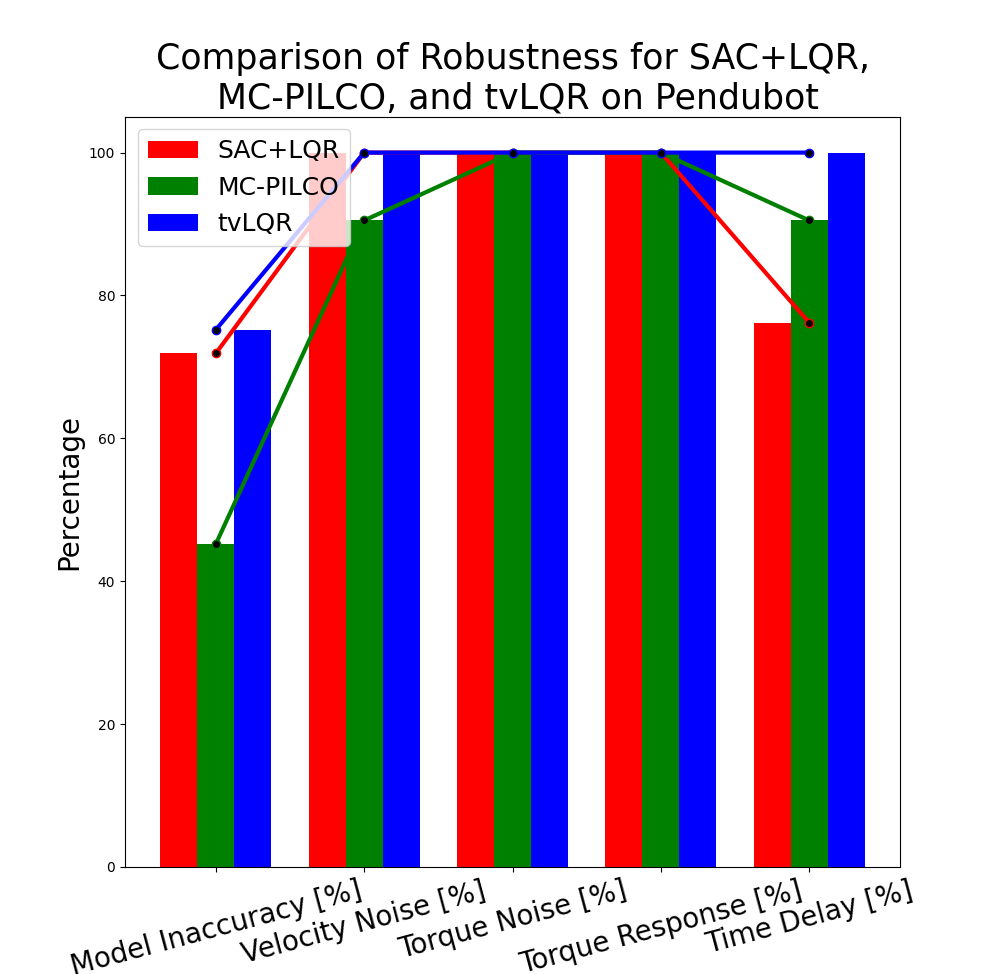
\includegraphics[width=0.47\textwidth]{figures/discussion/pendubot_robustness_bar.png}
% \hfill % This adds a space between the two figures
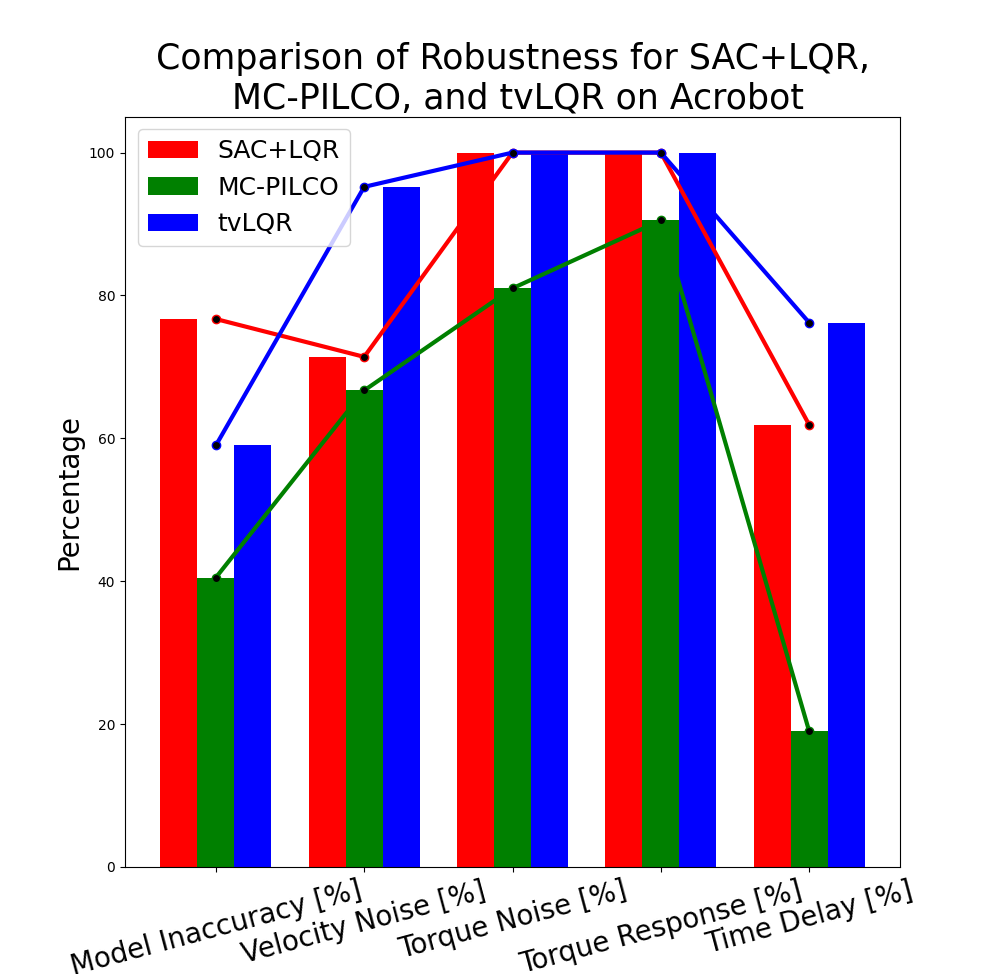
\includegraphics[width=0.47\textwidth]{figures/discussion/acrobot_robustness_bar.png}
\caption{Visualization of Robustness Scores on Pendubot and Acrobot}
\label{fig:robustness_visualization}
\end{figure}

In general, tvLQR achieves the best robustness scores for both pendubot and acrobot setups, followed by SAC+LQR, with MC-PILCO ranking last. While SAC+LQR boasts consistency in robustness across both setups, time delay remains a significant issue, limiting the robustness of RL-based methods.

\section{Interpretation of real system leaderboard}
The results of real system performance leaderboard is presented in Table \ref{tab:performance_real}. For the pendubot, SAC+LQR achieved a swing-up success rate of 40\%, while MC-PILCO had a perfect score of 100\%, and tvLQR scored 80\%. For the acrobot, SAC+LQR did not achieve success, MC-PILCO again scored 100\%, and tvLQR achieved full success as well. The swing-up time was fastest with SAC+LQR for the pendubot at 0.67 seconds, and for the acrobot, MC-PILCO had the fastest time at 1.55 seconds.

Apart from the swing-up time, MC-PILCO demonstrates superior performance on the pendubot, while tvLQR has the advantage for the acrobot. MC-PILCO's energy consumption on the pendubot is markedly lower, with marginally better maximum torque and a significant lead in integrated torque and torque cost metrics. The velocity cost further showcases MC-PILCO's high efficiency, contributing to its leading average RealAI score of 0.839.

\begin{table}[H]
  \centering
 \begin{tabular}{lcccccc}
 \hline
 Criteria & \multicolumn{2}{c}{SAC+LQR} & \multicolumn{2}{c}{MC-PILCO} & \multicolumn{2}{c}{tvLQR} \\
 & Pendubot & Acrobot & Pendubot & Acrobot & Pendubot & Acrobot \\
 \hline
 Swingup Success & 4/10 & 0/10 & 10/10 & 10/10 & 8/10 & 10/10 \\
 Swingup time [s] & \textbf{0.67} & - & 1.37 & \textbf{1.55} & 4.12 & 4.03 \\
 Energy [J] & 37.12 & - & \textbf{11.66} & 17.95 & 34.02 & \textbf{13.75} \\
 Max. Torque [Nm] & 5.0 & - & \textbf{4.99} & 5.0 & 5.0 & \textbf{2.98} \\
 Integrated Torque [Nm] & 24.87 & - & \textbf{3.72} & 5.93 & 19.06 & \textbf{5.61} \\
 Torque Cost [N²m²] & 78.7 & - & \textbf{8.93} & 11.73 & 51.88 & \textbf{3.26} \\
 Torque Smoothness [Nm] & 0.774 & - & \textbf{0.54} & 0.671 & 0.643 & \textbf{0.108} \\
 Velocity Cost [m²/s²] & 114.04 & - & \textbf{84.61} & 118.38 & 242.34 & \textbf{109.77} \\
 Best RealAI Score & 0.767 & - & \textbf{0.843} & 0.82 & 0.695 & \textbf{0.822} \\
 Average RealAI Score & 0.298 & - & \textbf{0.839} & 0.817 & 0.547 & \textbf{0.821} \\
 \hline
 \end{tabular}
 \caption{Real hardware performance scores of multiple controllers for pendubot and acrobot experiments.}
 \label{tab:performance_real}
\end{table}

In the acrobot trials, the scores are close between MC-PILCO and tvLQR. However, tvLQR outperformed MC-PILCO in terms of energy consumption and most torque-related criteria by a substantial margin. Additionally, tvLQR's torque smoothness is notably superior to that of MC-PILCO. tvLQR also achieved the highest average RealAI score of 0.821 for the acrobot.

In summary, while MC-PILCO displayed high efficiency and success rates for the pendubot, tvLQR excelled in torque smoothness and energy efficiency, particularly for the acrobot system. The SAC+LQR approach demonstrated rapid swing-up times for the pendubot but failed to register success for the acrobot.

\cleardoublepage
